% Homework template for Inference and Information
% UPDATE: September 26, 2017 by Xiangxiang
\documentclass[a4paper]{article}
\usepackage{amsmath, amssymb, amsthm}
% amsmath: equation*, amssymb: mathbb, amsthm: proof
\usepackage{moreenum}
\usepackage{mathtools}
\usepackage{url}
\usepackage{bm}
\usepackage{enumitem}
\usepackage{graphicx}
\usepackage{subcaption}
\usepackage{booktabs} % toprule
\usepackage[mathcal]{eucal}
%% Definitions for Inference and Information
%% UPDATE: 22/03/2018  by zhaofeng-shu33
%% This package does not require other packages
\ProvidesPackage{dtx-style}
% semester
\newcommand{\theterm}[1]{#1}
\newcommand{\thecourseinstitute}[1]{#1}
\newcommand{\thecoursename}[1]{\textsc{#1}}

\newcommand{\courseheader}[3]{
\vspace*{-1in}
\begin{center}
\thecourseinstitute{#1}\\
\thecoursename{#3} \\
\theterm{#2}
\vspace*{0.1in}
\hrule
\end{center}
}
\def\v#1{\underline{#1}}
\newcommand{\rvx}{\mathsf{x}}    % x, r.v.
\newcommand{\rvy}{\mathsf{y}}    % y, r.v.
\newcommand{\rvz}{\mathsf{z}}    % z, r.v.
\newcommand{\rvH}{\mathsf{H}} 
\newcommand{\uy}{\underline{y}}
\newcommand{\urvx}{\underline{\mathsf{x}}}    % x, r.v. vec
\newcommand{\urvy}{\underline{\mathsf{y}}}    % y, r.v. vec
\newcommand{\urvz}{\underline{\mathsf{z}}}    % z, r.v. vec
\newcommand{\urvw}{\underline{\mathsf{w}}} 
\newcommand{\defas}{\triangleq} %\coloneqq
\newcommand{\reals}{\mathbb{R}}
\newcommand{\TT}{\mathrm{T}}    % transpose
% \newcommand{\E}[1]{\mathbb{E}\left[{#1}\right]}
% \newcommand{\Prob}[1]{\mathbb{P}\left({#1}\right)}
\DeclareMathOperator*{\argmax}{arg\,max}
\DeclareMathOperator*{\argmin}{arg\,min}
\DeclareMathOperator*{\argsup}{arg\,sup}
\DeclareMathOperator*{\arginf}{arg\,inf}
\DeclareMathOperator{\diag}{diag}
\DeclareMathOperator{\Var}{Var}
\DeclareMathOperator{\Cov}{Cov}
\DeclareMathOperator{\MSE}{MSE}
\DeclareMathOperator{\In}{\mathbb{I}}
\DeclareMathOperator{\E}{\mathbb{E}}
\DeclareMathOperator{\Prob}{\mathbb{P}}
\newcommand\independent{\protect\mathpalette{\protect\independenT}{\perp}}
\def\independenT#1#2{\mathrel{\rlap{$#1#2$}\mkern2mu{#1#2}}}
\endinput

\begin{document}
\courseheader
\newcounter{hwcnt}
\setcounter{hwcnt}{6} % set to the times of Homework

\begin{center}
  \underline{\bf Homework \thehwcnt} \\
\end{center}
\begin{flushleft}
  赵丰\hfill
  \today
\end{flushleft}
\hrule

\vspace{2em}

\flushleft
\rule{\textwidth}{1pt}
\begin{itemize}
\item {\bf Acknowledgments: \/} 
  This coursework referes to wikipedia: \small{\url{https://en.wikipedia.org}}.

\item {\bf Collaborators: \/}
  I finish this coursework by myself.
\end{itemize}
\rule{\textwidth}{1pt}

\vspace{2em}

I use \texttt{enumerate} to generate answers for each question:

\begin{enumerate}[label=\thehwcnt.\arabic*.]
  \setlength{\itemsep}{3\parskip}

  \item 
    \begin{enumerate}[label=(\alph*)]
  \item 
  \begin{align*}
  \frac{p_{\urvy}(\uy;x)}{p_{\mathsf{t}(t(\uy);x)}} = & \frac{x^{y_1+y_2}(1-x)^{2-y_1-y_2}}{\binom{2}{y_1+y_2}x^{y_1+y_2}(1-x)^{2-y_1-y_2}} \\
  = & \frac{1}{\binom{2}{y_1+y_2}}
  \end{align*}
  上式与$x$无关,由Fisher-Neyman 因子定理得 $t(\uy)=y_1+y_2$ 是充分统计量。
  \item $\hat{x}(\underline{y})=y_1$ 是无偏估计量,MSE 等于Bernoulli 分布的方差,因此
  $\MSE_{\hat{x}}(x)=x(1-x)$
  \item   
    \begin{enumerate}[label=\roman*.]
  \item \textbf{因为}$\mathsf{t}$是充分统计量,$p_{\urvy| \mathsf{t}}(\uy|\mathsf{t}=t)$ 与$x$无关。
  所以
  \begin{align*}
     \hat{x}'(t) = & \E[\hat{x}(\urvy)|\mathsf{t}=t] \\
     = &\sum_{\uy} \hat{x}(\uy) p_{\urvy| \mathsf{t}}(\uy|\mathsf{t}=t)
  \end{align*}
  $\hat{x}'(t)$与$x$无关。
  \item
  沿用(a,b)中的假设,
  由对称性 $\E[\rvy_1|\mathsf{t}=t]=\E[\rvy_2|\mathsf{t}=t] \Rightarrow$
    $\hat{x}'(\mathsf{t})=\frac{\mathsf{t}}{2}$
    所以$\hat{x}'(\mathsf{t})$ 是无偏的,
    $\MSE_{\hat{x}'}(x)=\frac{1}{2}x(1-x)\Rightarrow$
    $\gamma=\frac{1}{2}$  
   \end{enumerate}
  \item 
    \begin{enumerate}[label=\roman*.]
    \item 由$\underline{\mathsf{t}}$是充分统计量可知。
    \item 
    \[
     \hat{x}'(\underline{t}) =  \sum_{\uy} \hat{x}(\uy) p_{\urvy| \underline{\mathsf{t}}}(\uy|\underline{\mathsf{t}}=\underline{t})
    \]
    由$C(x,\hat{x})$ 关于 $\hat{x}$的凸性以及概率质量函数的归一化特性可得:
    \[
    C(x,\hat{x}'(\underline{t})) \leq  \sum_{\uy} C(x,\hat{x}(\uy)) p_{\urvy| \underline{\mathsf{t}}}(\uy|\underline{\mathsf{t}}=\underline{t})
    \]
    $\Rightarrow$
    \begin{equation}\label{eq:61Mid}
    \sum_{\underline{t}} C(x,\hat{x}'(\underline{t}))p_{\underline{\mathsf{t}}}(\underline{t}) 
    \leq  \sum_{\uy,\underline{t}} C(x,\hat{x}(\uy)) 
    p_{\urvy| \underline{\mathsf{t}}}(\uy|\underline{\mathsf{t}}=\underline{t})p_{\underline{\mathsf{t}}}(\underline{t}) 
    \end{equation}
   因为
   $ p_{\urvy| \underline{\mathsf{t}}}(\uy|\underline{\mathsf{t}}=\underline{t})p_{\underline{\mathsf{t}}}(\underline{t}) 
   = p_{\urvy,\underline{\mathsf{t}}}(\rvy,\underline{t})=p_{\urvy}(y)\cdot 1_{\underline{t}=\underline{t}(y)} \Rightarrow$
   $\sum_{\underline{t}} p_{\urvy| \mathsf{t}}(\uy|\underline{\mathsf{t}}=\underline{t})p_{\underline{\mathsf{t}}}(\underline{t})
   =p_{\urvy}(y) $
   所以由\eqref{eq:61Mid}可得:
   \[
   \E[C(x,\hat{x}'(\underline{\mathsf{t}}))]\leq \sum_{\uy} C(x,\hat{x}(\uy)) 
    p_{\urvy}(y)
    =\E[C(x,\hat{x}(\urvy))]
   \]
   
%    \begin{align*}     
%    \end{align*}
   \end{enumerate}
  
   \end{enumerate}
  
  \item 
  \begin{enumerate}[label=(\alph*)]
  \item 
   \begin{align*} 
      \E_{\mathsf{x}|\mathsf{y}}[R(x,b_y)|\mathsf{y}=y] = & r(b_y)p_{\rvx|\rvy=y}(x=1)+r(1-b_y)p_{\rvx|\rvy=y}(x=0) \\
      \propto & (1+\ln(b_y))p\, p_{\rvy| \rvx=1}(y)+(1+\ln(1-b_y))(1-p) p_{\rvy| \rvx=0}(y)
   \end{align*}
   令$\frac{\partial R(x,b_y)}{\partial b_y}=0$,解得$b_y=
   \frac{p\,p_{\rvy| \rvx=1}}{p\,p_{\rvy| \rvx=1}+(1-p)p_{\rvy| \rvx=1}}=P_{\mathsf{x}|\mathsf{y}}(1|\mathsf{y}=y)$

   另解,设$\rvz\sim B(b_y)$:
   \begin{align*}
     \E_{\mathsf{x}|\mathsf{y}}[R(x,b_y)|\mathsf{y}=y] = & 1+ \ln 2(P_{\mathsf{x}|\mathsf{y}}(1|\mathsf{y}=y) \log P_{\rvz}(1) +\\
     + & P_{\mathsf{x}|\mathsf{y}}(0|\mathsf{y}=y)\log P_{\rvz}(0))\\
     = & 1-\ln 2(H(\rvx|\rvy=y)+D(\rvx|\rvy=y||\rvz))
   \end{align*}
   由相对熵的非负性,当$D(\rvx|\rvy=y||\rvz))$时回报的期望值最大,此时$b_y=P_{\mathsf{x}|\mathsf{y}}(1|\mathsf{y}=y)$
  \item
   \begin{align*} 
      R(x,b_y) = & r(b_y)p_{\rvx|\rvy=y}(x=1)+r(1-b_y)p_{\rvx|\rvy=y}(x=0) \\
      \propto & b_y p\, p_{\rvy| \rvx=1}(y)+(1-b_y)(1-p) p_{\rvy| \rvx=0}(y)
   \end{align*}
   令$\frac{\partial R(x,b_y)}{\partial b_y}=0$,解得
   \begin{equation}
      b_y=\begin{cases}
       0 & (1-p) p_{\rvy| \rvx=0}(y)>p\, p_{\rvy| \rvx=1}(y)\\
       1 & (1-p) p_{\rvy| \rvx=0}(y)\leq p\, p_{\rvy| \rvx=1}(y)
          \end{cases}
   \end{equation}
  \item
  \begin{enumerate}[label=\roman*.]
  \item 
   是  
  \item
   否
  \item
  与 $p$的取值和分布$p_{\rvy | \rvx }(\cdot | \cdot)$ 无关。
  \end{enumerate}

   \end{enumerate}    
  \item 
  \begin{enumerate}[label=(\alph*)]
  \item $\E_p[\rvy]=t \Rightarrow p_1+2p_2=t$
  若 $\E_p[\rvy]=0 \Rightarrow p_0=1,p_1=p_2=0$
  $\mathcal{L}_0=\{(1,0,0)\}$
  \item 当$t=\frac{1}{2}$时,$\mathcal{L}_{\frac{1}{2}}$是如图\ref{fig:d12}所示的线段。
    \begin{figure}[!ht]
    \centering
    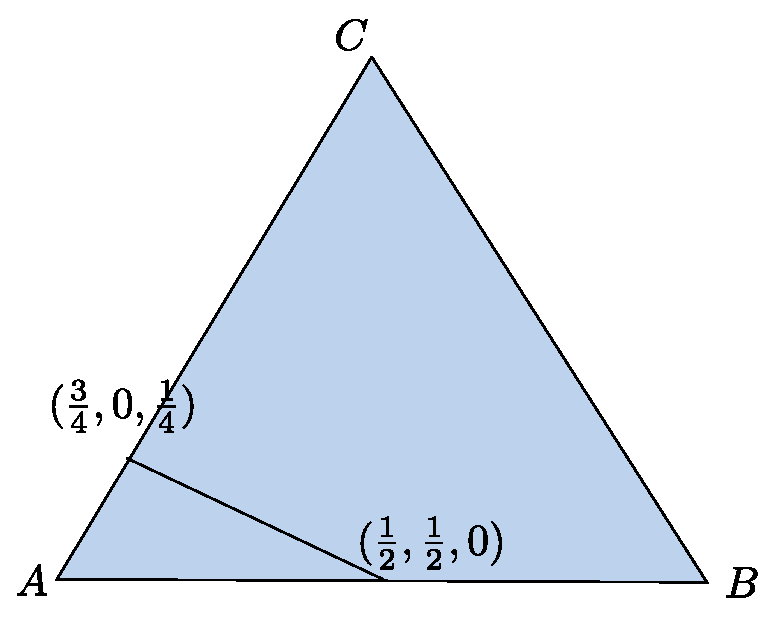
\includegraphics[width=5cm]{drawing.eps}
    \caption{$\mathcal{L}_{\frac{1}{2}}$}\label{fig:d12}
    \end{figure}
  \item 
  正交于$\mathcal{L}_{\frac{1}{2}}$的指数族$\mathcal{E}$上分布$q$可以写成如下的形式:
  \begin{equation}\label{eq:qpe}
        q(y)=p^*(y)e^{xy-\alpha(x)},y=0,1,2
  \end{equation}
  其中$p^*(y)\in \mathcal{L}_{\frac{1}{2}}$,它满足如下的方程:
  \begin{align}
   p^*(0)+p^*(1)+p^*(2)=& 1 \\
   p^*(1)+2p^*(2)=& \frac{1}{2} \\
  \end{align} 
  利用$q$点在指数族上,有如下比例关系:
  \[
   \frac{p^*(0)}{q(0)}=\frac{p^*(1)e^{x^*}}{q(1)}=\frac{p^*(2)e^{2x^*}}{q(2)}
  \]
  由上面四个等式可以解出$p^*=(\frac{2}{3},\frac{1}{6},\frac{1}{6})$
  在\eqref{eq:qpe}式中,当$x\to -\infty$时,由于$q(0)$衰减最慢及概率的归一化
  条件可得:$q_{x\to -\infty}=(1,0,0)$,同理可得$q_{x\to \infty}=(0,0,1)$
  指数族$\mathcal{E}$如图\ref{fig:d34}所示:
  \begin{figure}[!ht]
    \centering
    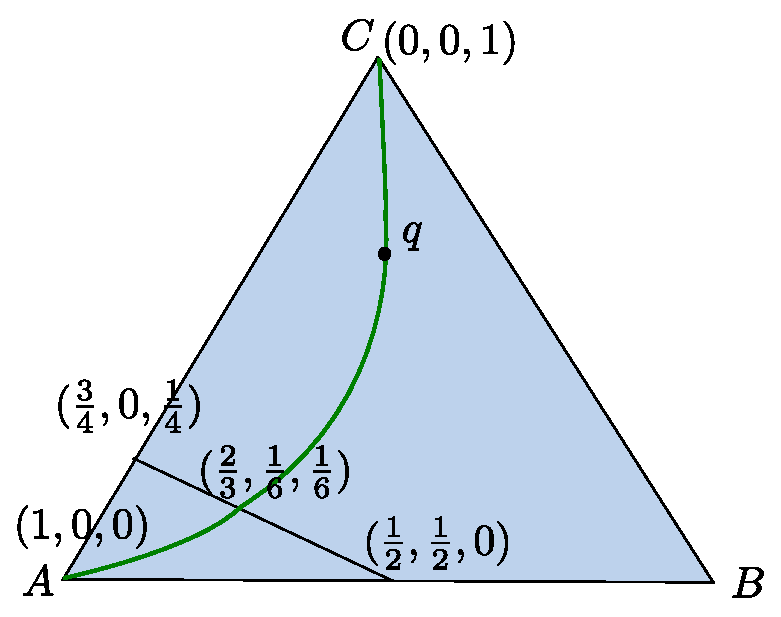
\includegraphics[width=5cm]{drawing2.eps}
    \caption{正交于$\mathcal{L}_{\frac{1}{2}}$的指数族$\mathcal{E}$}\label{fig:d34}
  \end{figure}
  \item (c) 中已求出 $p^*=(\frac{2}{3},\frac{1}{6},\frac{1}{6})$
  \item 区域$\mathcal{P}$如图\ref{fig:de}所示:
  \begin{figure}[!ht]
    \centering
    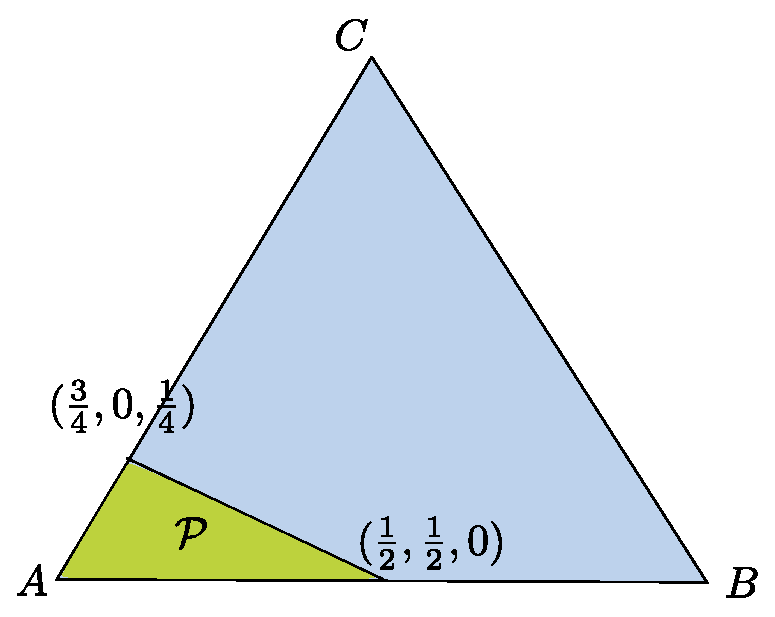
\includegraphics[width=5cm]{drawing3.eps}
    \caption{区域$\mathcal{P}$}\label{fig:de}
  \end{figure}
  \item 若$p^*$在区域$\mathcal{P}$内部取得,则由偏导数为0的性质推出$p^*=q$矛盾。
  因此只需分别考察$D(\cdot|| q)$ 在三角形区域$\mathcal{P}$的三条边上的取值,得到
  \[
   \argmin_{p \in \mathcal{P}} D(p||q) = (\frac{2}{3},\frac{1}{6},\frac{1}{6})
  \]
  与 (d) 的结果相同。
  \end{enumerate}
  
  \item Thanks to 陆石, who gives me this template.
  

  \end{enumerate}
\end{document}
\begin{equation}
\end{equation}

%%% Local Variables:
%%% mode: late\rvx
%%% TeX-master: t
%%% End:
